\documentclass[a4paper, 11pt, titlepage]{article}
\usepackage{fancyhdr}
\usepackage{graphicx}
\usepackage{imakeidx}
\usepackage{makeidx}
\usepackage{mathtools}
\usepackage[spanish]{babel}
\usepackage{eurosym}
\usepackage{hyperref}
\usepackage{amssymb}
\usepackage{listings}
\usepackage{xcolor}

% \setcounter{secnumdepth}{5}
% \setcounter{tocdepth}{5} 

\title{Inteligencia artifical}
\author{Francisco Javier Balón Aguilar}

\begin{document}

\maketitle
\renewcommand{\contentsname}{Índice}
\tableofcontents
\newpage 

\section{Contextualización}

    La inteligencia artifical puede definirse como una rama de la computación dedicada al
    desarrollo de agentes inteligentes no vivos por medio de las técnicas de la computación 
    y la programación.

    \paragraph{Etapa anterior al siglo XX} Las bases en las que se apoya el desarrollo de la inteligencia 
    artificial son anteriores al siglo XX, concretamente podemos ver su origen en la antigua Grecia.

    Aristóteles hacia el año 300 a.C. ya definió, en sus estudios, lo que conocemos como 
    \textbf{silogismos}\footnote{
        Un silogismo es un conjunto estructurado de reglas que describen una parte del conocimiento, 
        a partir de las cuales se pueden establecer conclusiones racionales en base a unas 
        premisas dadas.
    }. Posteriormente, hacia el año 1.315, Ramón Llull, basándose en otra herramienta astrológica 
    árabe, para combinar conceptos mecánicamente. Esta máquina estaba formada por tres discos 
    giratorios concéntricos que albergaban regiones en las que se ubicaban determinadas categorías 
    del pensamiento; es decir, girando estos discos se formaban nuevas teorías (véase imagen 
    \ref{arsmagna}).

    \begin{figure}[htp]
        \centering
        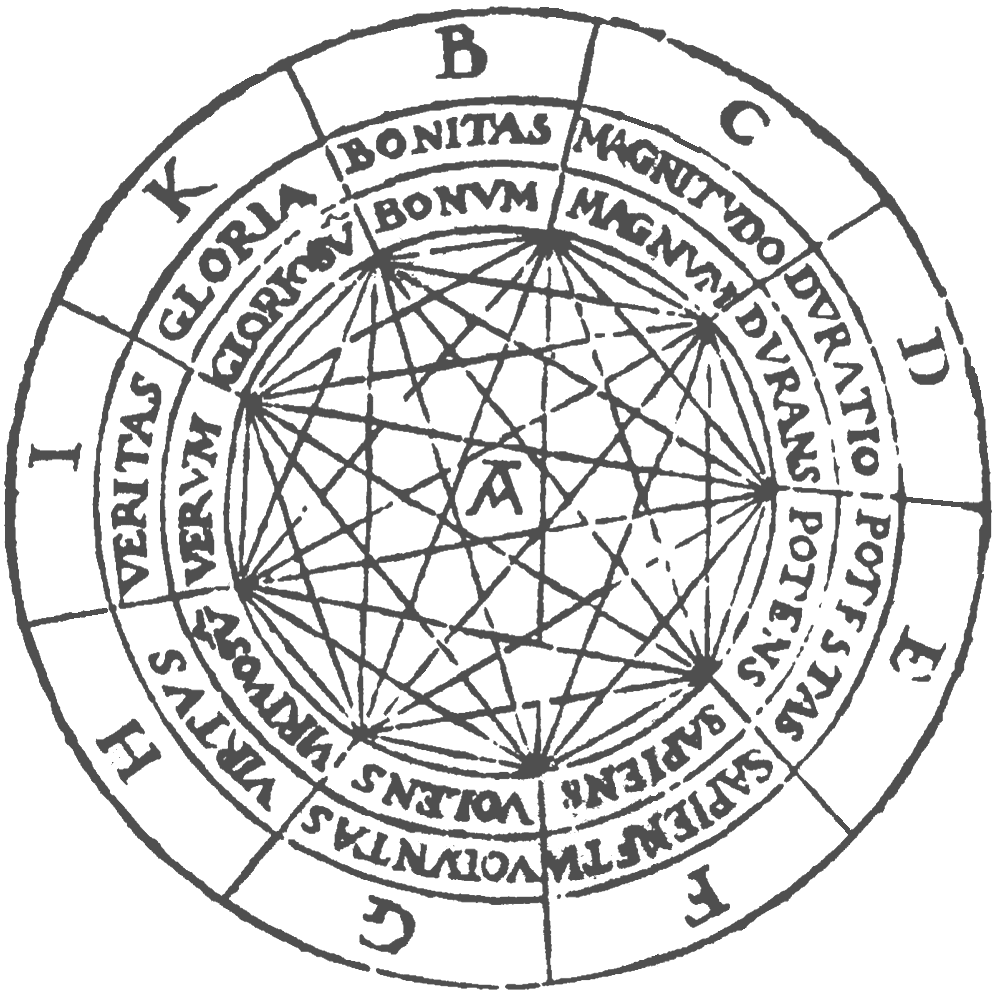
\includegraphics[width=0.4\textwidth]{resources/arsmagna.png}
        \caption{Esquema de la máquina Ars Magna, de Ramón Llull.}
        \label{arsmagna}
    \end{figure}

    En el año 1.842, Charles Babbage es considerado el padre de la informática por la creación de la 
    primera calculadora mecánica programable (véase imagen \ref{maquinabaggage}), introduciendo las bases 
    de la computación.

    \begin{figure}[htp]
        \centering
        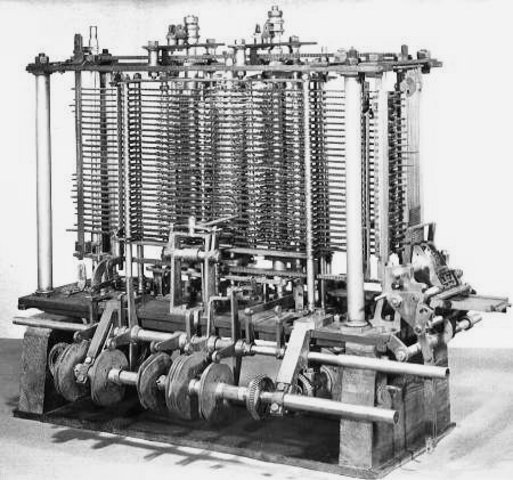
\includegraphics[width=0.6\textwidth]{resources/maquinababbage.jpg}
        \caption{Máquina analítica de Babbage.}
        \label{maquinabaggage}
    \end{figure}

    Unos años más tarde, en 1.847, George Bool con su llamada lógica booleana o proposicional, mientras 
    investigaba las leyes fundamentales sobre las que basa el razonamiento humano y su expresión matemática, 
    añadió complejidad a la lógica de Aristóteles. Basándose en estos estudios, en 1.879, Gottlob Frege extiende 
    la lógica booleana creando la lógica de Primer Orden, utilizada hasta nuestros días y con una escalabilidad 
    de expresión mayor que la lógica booleana.

    \paragraph{El siglo XX} El desarrollo de la computación alrededor de los años 40 supuso un impulso exponencial 
    para el desarrollo de la inteligencia artificial como ciencia. El primero en vaticinarlo fue Alan Turing, en
    1.950, introduciendo la posibilidad de mecanizar la inteligencia humana a través de una evolución de su máquina 
    de Turing (simultáneamente propuso el conocido test de Turing, o juego de imitación, a través del cual las 
    máquinas llegarían a emular el comportamiento humano inteligente a base de preguntas y razonamientos mecánicos).

    Si podemos dar un <<nacimiento>> a la inteligencia artificial en la práctica podemos considerarlo en el verano 
    de 1.956, en un evento en el Dartmouth College en New Hampshire. Tal evento estuvo organizado por John McCarthy, 
    creador del lenguaje LISP, Marvin Minsky, Nathaniel Rochester y Claude Shanon. Este mismo año se desarrollaron en 
    IBM (con Nathaniel Rochester) algunos de los primeros programas considerados como <<inteligentes>>, como juegos 
    de damas (con Claude Shanon) o un demostrador de teoremas de geometría (Gelernter).

    Un programa que llamó la atención en 1.966 fue ELIZA, por Joseph Weizenbaum. Éste permitía establecer una 
    conversación simple entre el ordenador y el humano.

    En los años 70 aparecieron dos proyectos que captaron la atención del gremio. El primero fue el sistema SHRDLU, 
    desarrollado por Terry Winograd, del Instituto Tecnológico de Massachussets (MIT). Este sistema suministra 
    una interfaz de lenguaje natural al brazo de un robot acerca de un conjunto de objetos que aparecen en pantalla y 
    los movimientos que se pueden realizar con ellos. El segundo fue el sistema LUNAR de William Woods, que proporciona 
    a los geólogos lunares una interfaz en lenguaje natural que permite acceder a una base de datos de rocas lunares. 

    %TODO: ¿seguir o no seguir?

\section{Sistemas de representación del conocimiento}

    Resulta un problema plasmar las formas de expresión humana a nivel computacional, especialmente
    por la complejidad de éstas. De esta necesidad surgen los modos de esquematización del 
    conocimiento, disminuyendo la pérdida de información en el proceso.

    Los sistemas de representación de conocimiento deben garantizar los objetivos:

    \begin{itemize}
        \item \textbf{Idoneidad del sistema de representación}. El sistema debe ser capaz de 
        englobar toda la información relevante para la resolución del problema, siempre de una 
        forma sencilla y simplificada.
        \item \textbf{Adecuación inferencial}. A partir de un coste computacional no muy elevado,
        la manipulación y combinación de las estructuras del sistema deben inferir conocimiento 
        nuevo a partir del ya existente.
        \item \textbf{Capacidad de crecimiento}. El sistema debe ser suficientemente flexible y 
        escalable para la incorporación de nuevas estructuras y conocimiento.
    \end{itemize}

    Otros factores a tener en cuenta, quedando éstos en segundo plano, son el nivel de detalle 
    en la representación del conocimiento, la facilidad de reconocimiento de conocimiento 
    representado o la posibilidad de cambiar la representación del conocimiento en su forma 
    origen.

    Para contextualizar en su aplicación, podemos agrupar en cuatro los modelos más utilizados 
    teniendo en cuenta las características expuestas:

    \begin{itemize}
        \item \textbf{Esquemas de representación lógica}. Véase sección \ref{esquemasrepresentacionlogica}.
        \item \textbf{Esquemas de representación procedural}. El conocimiento es representado 
        como un conjunto de instrucciones mediante las cuales se resuelven problemas.
        \item \textbf{Esquemas de representación en forma de malla o red}. El conocimiento 
        es representado en forma de grafos, donde cada nodo es un objeto del problema a 
        resolver y los arcos pueden interpretarse como relaciones entre los objetos.
        \item \textbf{Esquemas de representación estructurada}. Amplía la representación 
        conceptual en forma de malla, permitiendo a cada nodo estructurarse de forma más 
        compleja, como una estructura de datos con un conjunto de atributos y valores.
    \end{itemize}

    \subsection{Esquemas de representación lógica}\label{esquemasrepresentacionlogica}

        Los esquemas de representación lògica como el cálculo de proposiciones o la lógica 
        de primer orden son muy utilizados en disciplinas como la Ingeniería del Conocimiento, 
        utilizada para crear \textit{sistemas expertos}\footnote{
            Un sistema experto, es un sistema informático que emula el razonamiento humano 
            actuando tal y como lo haría un experto en un área de conocimiento. 
        }.

        La lógica está compuesta por cálculos, definiéndose como una estructura o sistemas 
        de relaciones que conforman algo similar a un lenguaje, de tal forma que se 
        compongan de:

        \begin{itemize}
            \item Símbolos, que representan cada parte de la información.
            \item Reglasde formación de expresiones, que rigen la combinación de Símbolos 
            para conformar expresiones.
            \item Reglas de transformación, que conjuntan las directrices que indican el 
            protocolo de transformación de una expresión a otra.
        \end{itemize}

        \subsubsection{Lógica de enunciados}\label{logicaenunciados}

            La lógica de enunciados se presenta como la representación más simple dentro de la 
            lógica formal. Trata el estudio de los enunciados a través de conectores, estudiando 
            su veracidad o falsedad: según el \textit{principio de bivalencia} un enunciado 
            no puede ser verdadero y falso a la vez.

            Se forma por proposiciones, que son enunciados de los que se puede disponer de un 
            criterio de veracidad o falsedad, y que deben estar por un lado bien formulados, 
            y por otro debe haber una afirmación. De tal manera que los enunciados por oraciones
            (representadas por simbolos como $p$, $q$, $r$, $s$, $t$, etc.) 
            y partículas que enlazan dichas oraciones.

            Por ejemplo, en la sentencia <<Si llueve, me mojo>>, se podría formalizar como 
            $p$ (llover), $q$ (mojarse) y representar la oración tal que: <<Si $p$ entonces $q$>>

            Por otro lado las oraciones necesitan conectivas que establezcan una relación entre 
            los símbolos, como:

            \begin{itemize}
                \item Negación ($\neg$). P. Ej: Siendo $p$ <<llover>>; $\neg p$ es <<no llueve>>.  
                \item Conjunción ó \textit{AND} ($\land$). P. Ej: $p\land q$ es <<llueve y me mojo>>.
                \item Disyunción ó \textit{OR} ($\lor$). P. Ej: $p\lor q$ es <<llueve o estudio>>.
                \item Implicación. Se produce cuando la ejecución de una acción lleva a otra relacionada.
                P. Ej: $p\Rightarrow q$ puede entenderse como <<llueve, ergo me mojo>>, derivando $q$ 
                de $p$.
            \end{itemize}

            \paragraph{Modelación compleja con conectivas} 
            
                Como es de suponer, las conectivas citadas pueden ser combinadas para modelar sentencias 
                más complejas. P. Ej:

                Siendo: $p=$ lluvia; $q=$ refresca; $r=$ terminación de problemas de sequía; $t=$
                necesidad de mayor inversión:
                
                \[p \lor q \Rightarrow (r \land \neg t)\]

                Ó <<Si llueve o refresca, se terminarán los problemas de sequía y no habrá necesidad 
                de mayor inversión>>.

                Siendo: $p=$ acepto el mundo que me ofrecen; $q=$ soy feliz; $r=$ empiezo a cavar 
                mi propia tumba; $s=$ no veo la posibilidad de cambiar este mundo:

                \[[(p \land q) \Rightarrow r] \lor [(\neg q \land s) \Rightarrow r]\]

                Ó <<Si acepto el mundo que me ofrecen y soy feliz así, entonces empiezo a cavar mi 
                propia tumba; o bien, si no soy feliz así, y no veo tampoco posibilidad de cambiar 
                ese mundo, emprendo asimismo mi enterramiento>>.

                Cabe destcar que el lenguaje natural permite una expresividad muy amplia a la hora de 
                transmitir información, por lo que en determinadas ocasiones puede complicar la 
                formializción de enunciados. Es necesario pues simplificar la información englobada en 
                cada variable, eliminando giros lingüisticos, formalismos y otros elementos que 
                sobrecargan estas expresiones.

            \paragraph{Asignación de valores de verdad a proposiciones}

                La verdad o falsedad de una proposición se calcula a través de la descomposición
                de sus conectivas lógicas. Para ello se utilizan las tablas de verdad propias del 
                Álgebra de Boole. 

                % TODO: Tablas de verdad

    \subsection{Lógica de predicados}

        Trata del estudio y profundización de las frases y su estructura interna de las proposiciones, 
        siendo ésta fundamentada en la lógica de enunciados (véase sección \ref{logicaenunciados}).

        Es necesaria la identificación primera de todos los individuos y sus predicados, es decir, 
        relaciones y propiedades entre estos individuos, ofreciendo los siguientes símbolos:

        Dentro de la lógica de predicados existen las \textit{funciones de enunciado}, donde se expresa 
        de forma genérica y a través de variables un enunciado, el cual cobrará sentido una vez se 
        identifique el valor de las variables.

        \paragraph{Funciones de enunciado}

            Dentro de la lógica de predicados existen las funciones de enunciado, donde éstos son 
            expresados de forma genérica y a través de variables, y en la que cada variable representa 
            un individuo. Dependiendo de los valores por los que se sustituyan la variable, el enunciado 
            será verdadero o falso.

            Dentro de las expresiones formalizadas pueden aparecer \textit{cuantificadores}, 
            modificadores lingüisticos que indican el número de individuos que comparten cierta propiedad.

            En el presente documento estudiaremos dos tipos de cuantificadores:

            \begin{itemize}
                \item Cuantificador universal. Se representa con el símbolo $\forall$ y se traduce como 
                <<para todo>> o <<todo>>. P. Ej: $\forall x hombre(x)\Rightarrow mortal(x)$ ó <<todos los hombres 
                son mortales>>, simplificado como <<los hombres son mortales>>.
                \item Cuantificador existencial. Se representa con el símbolo $\exists$ y se traduce como 
                <<algunos>> o <<no todos>>. P. Ej: $\exists x hombre(x) \land bueno(x)$ ó <<algunos hombres 
                son buenos>>, o dicho de otro modo <<no todos los hombres son buenos>>.
            \end{itemize}

            Cabe destacar que el símbolo que se utiliza para negar cuantificadores es $\rceil$, siendo 
            $\forall x \rceil P(x)$ ó <<ningún elemento $x$ cumple $P$>>. P. Ej: 
            $\exists x, rio(x) \land \rceil suena(x)$ ó <<algunos ríos no suenan>>.

    \subsection{Esquemas de representación basados en redes semánticas}
        
        En el modelo de red semántica\footnote{
            Las redes semánticas se utilizan para representar mapas conceptuales, relacionando 
            unos conceptos con otros.

            Surgieron a través de los trabajos de Novak en la Universidad de Cornell.
        } los conceptos y las relaciones entre ellos quedan 
        representados a través de un grafo, pudiendo entonces plasmarse generalmente en forma 
        de árbol o grafos dirigidos.

        Este modelo tiene como núcleo el modo de relación entre los objetos y no la veracidad 
        o falsedad de una proposición. Así, la representación conceptual consta de una serie de 
        nodos (objetos) y una serie de arcos (relaciones) que contienen el nombre de la relación
        (véase figura \ref{graforedsemantica}), y creando una jerarquía que vaya desde las 
        formas de definición más generalistas hasta las más particulares.

        \begin{figure}[htp]
            \centering
            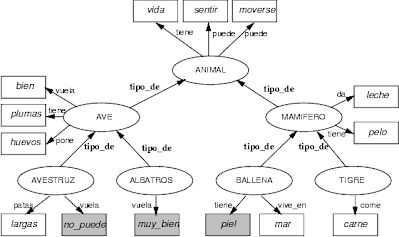
\includegraphics[width=0.8\textwidth]{resources/graforedsemantica.png}
            \caption{Ejemplo de grafo funcional en red semántica.}
            \label{graforedsemantica}
        \end{figure}    

\section{Procesos basados en reglas}

    \subsection{Razonamiento en Inteligencia Artificial}

        Como hemos visto anteriormente, el objetivo de los sistemas de representación lógica, es 
        generar nueva información a través de la obtenida en función de los enunciados. Esta capacidad 
        de aprendizaje mediante conocimiento obtenido se denomina \textbf{estrategia de inferencia}.

        El \textbf{razonamiento} se puede definir como el mecanismo por el cual dadas unas 
        condiciones iniciales, se obtiene una serie de conclusiones o hechos a través de un proceso 
        de deducción o inferencia. Estos modelos de razonamiento forman parte de los sistemas 
        lógicos y constan de un conjunto de reglas bien definidas que se utilizarán como argumentos 
        en los procesos de inferencia.

    \subsection{Cálculo lógico}\label{calculologico}

        El cálculo lógico se define como el proceso que permite obtener nuevos enunciados a 
        partir de otros verdaderos, de tal forma que un proceso de inferencia sea una operación (o 
        aplicación de una serie de operaciones lógicas) que obtenga una conclusión a partir de las 
        premisas dadas y mediante las reglas de inferencia ya establecidas.

        \subsubsection{Inferencia mediante deducción natural y relaciones de equivalencia}

            Este método utiliza dos reglas de inferencia para cada conectiva, sirviendo una para 
            insertarla y otra para eliminarla.

            Existen numerosas relaciones de equivalencia que se pueden aplicar para resolver 
            o simplificar enunciados, siendo las más importantes:

            \paragraph{Complemento, $\neg(\neg A) = A$} ó <<la negación de una negación da como 
            resultado una afirmación>>; $-(-1) = 1$.

            \paragraph{Idempotente, $A \lor A = A; A \land A$} Esta relación se aplica cuando 
            aparece la conjunción o disyunción del mismo enunciado, por lo que se obtendrá como 
            resultado la validez del mismo.


            \paragraph{Primera Ley de DeMorgan, $\neg (A \land B) = \neg A \lor \neg B$} Indica 
            que <<la negación de una conjunción es equivalente a la disynción de cada uno de sus 
            términos negados>>.             
            
            \paragraph{Segunda Ley de DeMorgan, $\neg (A \lor B) = \neg A \land \neg B$} Indica que 
            <<la negación de una disyunción es equivalente a la conjunción de cada uno de sus 
            términos negados>>.

            \paragraph{Distributiva, $P \lor (Q \land R) = (P \lor Q) \land (P \lor R)$} Afecta 
            a una conjunción de enunciados, de tal forma que equivaldría a la conjunción de sus 
            disyunciones.

            \paragraph{Conmutativa, $P \lor Q = Q \lor P$} Se aplica a la conjunción y a la 
            disyunción, no a las implicaciones.

            \paragraph{Implicación, $A \Rightarrow B = \neg A \lor B$} En una implicación, 
            siempre que se da el antecedente, se deriva el consecuente; por lo que en una 
            situación dada, o se produce el antecedente y por tanto la implicación $A \Rightarrow B$,
            se obtendría $B$ también, de lo contrario, no se habrá llegado a producir $A$, por lo 
            que se debe dar o bien $A$, por lo que en todo caso se deber dar o bien $A$ 
            (con lo que se obtendría $B$), o $\neg A$.

            \paragraph{Implicación, $A \Rightarrow B = \neg B \Rightarrow \neg A$} Si un antecedente 
            implica un consecuente, la negación del consecuente lleva asociado que no se ha producido 
            el antecedente; su negación.

            \paragraph{Modus Ponens, $(A \Rightarrow B) \land A = B$} Si en una implicación se tiene el 
            antecedente, también se tiene el consecuente como resultado de la implicación. 

            \paragraph{Modus Tollens, $(A \Rightarrow B) \land \neg B = \neg A$} Se refiere a la negación 
            del consecuente en una implicación; si no se da el consecuente es porque el antecedente 
            no se ha producido. De tal forma que, en una implicación, si se tiene además la negación 
            del consecuente, se puede derivar la negación del antecedente.

            \paragraph{Regla de la cadena} Si se tienen varias implicaciones de tal manera que $A \Rightarrow B$, 
            y a su vez $B \Rightarrow C$, entonces se infiere conclusión que $A \Rightarrow C$.

    \subsection{Métodos de demostración}

        En particular, el objeto de estudio serán los métodos deductivos, fundamentadas en una 
        serie de hipótesis partiendo de un conocimiento global y general, y particularizadas para 
        un caso dado.

        En los métodos deductivos, las premisas se denominan \textit{axiomas}, y son enunciados 
        o proposiciones verdaderas en sus afirmaciones. Estos métodos están formados por 
        \textit{silogismos}\footnote{
            Dado por Aristóteles, se define como una forma de razonamiento deductivo que está 
            formado por dos o más proposiciones como premisas y otra que se deriva de las anteriores 
            como conclusión.
        }

        \subsubsection{Demostración por el método directo}

            Dado un conjunto de premisas, suponemos una hipótesis (\textit{hipótesis auxiliar}), a 
            partir de la cual y tomando como referencia las reglas del razonamiento lógico (véase 
            sección \ref{calculologico}), se puede establecer una conclusión (o la validez de una 
            proposición dada).

        \subsubsection{Demostración por el método de reducción al absurdo}

            Se introduce como premisa la negación de aquello que se quiere demostrar, de tal 
            forma que si se obtiene como conclusión una contradicción, se demuestra que la premisa 
            que hemos introducido es falsa, por lo tanto su negación será verdadera.

            Es un método de resolución indirecto, ya que debemos partir de una suposición.

    \subsection{Métodos de encadenamiento hacia delante y hacia atrás}

        \subsubsection{Ecadenamiento hacia delante (Forward chaining)}

            Se parte de una serie de hechos iniciales, donde a través del conjunto de reglas se 
            obtienen nuevas conclusiones, estando condicionadas éstas por los datos iniciales.

            Los hechos se almacenan en la memoria de trabajo. Las reglas del sistema representan 
            posibles acciones que se pueden disparar cuando se cumplen determinadas condiciones
            en los hechos de la memoria de trabajo, y cada acción disparada suele implicar la adición 
            o supresión de loshechos en la memoria de trabajo. De esta forma, el sistema primero 
            localiza aquellas reglas relacionadas con los hechos, seleccionando una y ejecutando la 
            acción reflejada en la regla. Esta selección de la regla a disparar no es trivial y 
            pueden exstir numerosos factores que condicionen el orden de ejecución (prioridades), 
            por lo que existen estrategias de resolución de conflictos.

        \subsubsection{Encadenamiento hacia atrás (Backwards chaining)}

            Siendo éste el proceso inverso, se parte de un conjunto de síntomas y se buscan 
            las causas que las provocan.

            Se parte de una hipótesis que se trata de validar reconstruyendo la cadena de 
            razonamiento en orden inverso, de tal forma que se van añadiendo nuevas hipótesis 
            a validar hasta que se demuestre la hipótesis inicial.

            Se suelen utilizar sistemas de diagnóstico, donde dadas unas hipótesis, se deben 
            encontrar las reglas que las verifiquen.

            \begin{figure}[htp]
                \centering
                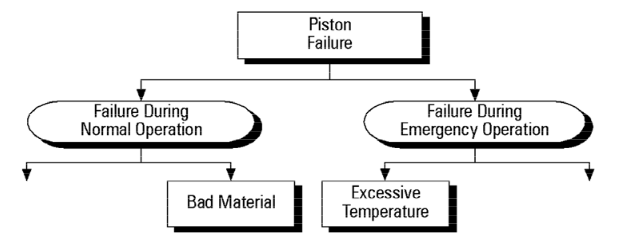
\includegraphics[width=0.8\textwidth]{resources/backwardschaining.png}
                \caption{Ejemplo gráfico de razonamiento hacia atrás por el fallo de un pistón.}
                \label{backwardschaining}
            \end{figure}    

    \subsection{Árboles de decisión}

        \subsubsection{Aprendizaje automático}

            El aprendizaje automático es una rama de la Inteligencia Artificial que se encarga 
            del diseño y desarrollo de algoritmos capaces de obtener nuevo conocimiento y de 
            organizarlo con el ya existente.

            Las técnicas de aprendizaje automático son modelos en constante desarrollo y evolución, 
            que necesitan estar constantemenet actualizados\footnote{
                El aprendizaje automático es fundamental en determinadas áreas como en la construcción 
                de sistemas expertos que requieran constante actualización de datos para mantenerse útiles.
            }.

            Éste puede ser clasificado en:

            \begin{itemize}
                \item \textbf{Aprendizaje supervisado}. Se parte de un conjunto de ejemplos 
                donde un mecanismo externo (generalmente humano) proporciona información sobre 
                la correcta clasificación para los textos (anotación o etiquetado). Los mecanismos 
                que se suelen aplicar son \textit{Reconocimiento de patrones (Pattern recognition)}
                y \textit{Aprendizaje automático (Machine learning)}, utilizados ampliamente en 
                clasificación sueprvisada en clasificadores estadísticos.
                \item \textbf{Aprendizaje no supervisado}. La clasificación debe realizarse sin 
                ninguna referencia a información externa, estando basada generalmente en técnicas 
                de \textit{clustering (agrupamiento)} y similares.
            \end{itemize}

            Esta evolución ha dado lugar a distintos \textbf{tipos de paradigma asociados al 
            aprendizaje}, dividiéndose en:

            \begin{itemize}
                \item \textbf{Paradigma analógico}. Se basa en encontrar una solución a un problema 
                utilizando uno ya resuelto ed planteamiento similar, de tal forma que por analogía si 
                dos problemas son similares en su planteamiento; también lo deben ser en sus conclusiones.
                
                De tal forma que debemos disponer de:

                \begin{itemize}
                    \item \textbf{Problema base}. Problemas ya resueltos que sirven de modelo. 
                    \item \textbf{Dominio base}. Ámbito de conocimiento en el que se define 
                    el problema base.
                    \item \textbf{Problema objetivo}. Problema planteado a resolver.
                \end{itemize}

                \item \textbf{Paradigma conexionista}. Se basa en la simulación del cerebro 
                humano con objetivo de recrear su actuación --enfocándose en modelos biológicos--, 
                conectando unidades simples entre sí.

                Parte de un conjunto de unidades de procesamiento simple (\textit{neuronas}) 
                que interactúan entre sí a través de \textit{conexiones}. Para que una neurona 
                se active debe superar un umbral de activación marcado, tal que en función de 
                las entradas recibidas, transmitirá una información de salida a todas las neuronas 
                que estén conectadas a ella.
                
                \item \textbf{Paradigma evolutivo}. Los algoritmos enmarcados en este paradigma, 
                aprenden simulando los mecanismos presentes en la evolución y la naturaleza, siendo 
                un referente en el paradigma los \textit{algoritmos genéticos}. 

                Los resultados son <<mejorados>> en cada iteración a través de conjuntos de 
                individuos (variables) seleccionados en cada iteración, lo que conlleva una serie 
                de casos:

                \begin{itemize}
                    \item \textbf{Proceso de inicialización}. Se selecciona aleatoriamente 
                    la población inicial de elementos (\textit{cromosomas}) que pueden constituir
                    parte de la solución del problema, debiendo ser suficientemente heterogénea 
                    para permitir una serie de iteraciones.
                    \item \textbf{Proceso de evaluación}. Cada cromosoma debe ser evaluado para 
                    conocer la \textit{bondad} de la solución.
                    \item \textbf{Reproducción}. Selección, cruce y mutación de población.
                    \item \textbf{Condición de parada}. Puede estar marcada por un número 
                    de iteraciones predefinidas, o porque la solución encontrada en una de 
                    ellas es suficientemente buena como para no seguir iterando.
                \end{itemize}

                \item \textbf{Paradigma inductivo}. Se basa en la evidencia empírica, obteniendo 
                la resolución de un conjunto de ejemplos que lo afirman y otro que lo niegan, 
                estableciendo características comunes de los conjuntos que representan un concepto.

                En conclusión, a partir de un conjunto de ejemplos, obtener un modelo de estructura
                que los clasifique bien con el menor ruido posible (errores en la estimación de un 
                atributo), y que realice entonces predicciones correctas. 

                Un árbol de decisión es una organización jerárquica que permite la clasificación 
                de un conjunto de atributos en una serie de clases que los defina e identifique, 
                componiéndose de:
                
                \begin{itemize}
                    \item \textbf{Atributos}. Características de un conjunto de objetos que establecen 
                    particiones.
                    \item \textbf{Nodos}. Respuestas a una pregunta que se formula para dividir los ejemplos.
                    \item \textbf{Ramas de un nodo o arcos}. Interconexiones del grafo entre los nodos.
                \end{itemize}
                
                Es necesario establecer un criterio para escoger un atributo dentro del conjunto que sirva como 
                separador, de tal forma que, a través de sucesivas iteraciones, se va formando el árbol. 
                Utilizando los separadores como nodos y los ejemplos como hojas de éste.

                \begin{figure}[htp]
                    \centering
                    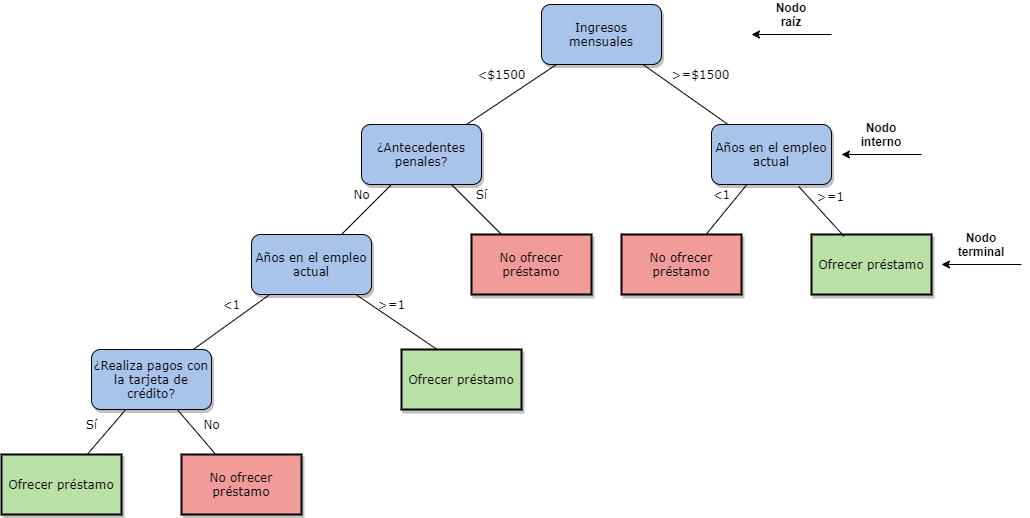
\includegraphics[width=0.8\textwidth]{resources/arbol-decision.png}
                    \caption{Ejemplo de árbol de decisión.}
                    \label{arboldecision}
                \end{figure}    
        
                En la creación de un árbol de decisión (véase figura \ref{arboldecision}), se tiene un 
                nodo raiz, nodos intermedios, y hojas. Cada hoja del árbol contiene un conjnto de ejemplos 
                representados por una sola clase\footnote{
                    Dentro de una hoja puede haber ruido, o ejemplos que no cumplan las características 
                    al $100\%$.
                }. La clase se establece en función de la mejor separación donde pertenezcan la mayoría, 
                o un número elevado de ejemplos.

            \end{itemize}

        \subsubsection{Algoritmo ID3}

            El algoritmo ID3 (\textit{Induction Decision Trees}) fue creado por \textit{Ross Quinlan} en 
            1986. Este algoritmo se basa en el principio denominado <<navaja de Occam>>, es decir, la solución 
            más simple y evidente es la acertada. De tal forma que crea árboles de decisión lo más compactos 
            posible en función de unos criterios de coste y bondad.

            Como desventaja fundamental que presenta, es que favorece la elección de aquellos atributos que contienen 
            muchos valores, lo que no siempre es lo más útil.

            El algoritmo de ID3 es un proceso recursivo, que se repite de manera iterativa hasta que llegar a un punto 
            de parada. Siendo sus características principales:

            \begin{itemize}
                \item El objetivo es producir un árbol de decisión que clasifique corréctamente 
                todos los ejemplos en subconjuntos de elementos del conjunto de entrenamiento.
                \item El árbol se genera dividiendo sucesivamente el conjunto de aprendizaje en 
                subconjuntos de ejemplos cada vez más pequeños hasta conseguir conjuntos de elementos 
                suficientemente puros.
                \item Es una partición recursiva del espacio de entradas en zonas homogéneas o puras 
                a la que se asocia una clase.
                \item El conjunto es bastante puro cuando casi todos sus ejemplos pertenecen a una sola
                clase.
            \end{itemize}

            Para conseguir el mejor separador, se deben tener en cuenta además las siguientes 
            consideraciones:

            \begin{itemize}
                \item Un separador es un solo atributo, otorgando significado físico y sencillez 
                de interpretación. Cada atributo dará lugar a un nodo intermedio donde sus hojas 
                son las clases.
                \item Es necesario usar una medida de distinción entre candidatos. 
                \item Esta medida se basa en la entropía.
            \end{itemize}

            La entropía se puede definir como la cantidad de información que hay dentro de un nodo, 
            siendo necesario el cálculo de entropía de cada uno de los posibles separadores.

            \[I(N)=-\displaystyle\sum_{i=1,Nclases} p(N,C_i) log_2 [p(N,C_i)]\]

            Donde $N$ es el número de clases diferentes en el nodo y $p(N, C_i)$ es la proporción 
            de ejemplos en el nodo perteneciente a la clase $C_i$.

            Cuanto más homogéneo sea el grupo más proporción de elementos de una sola clase habrá en él, 
            y por lo tanto menor será su entropía; siendo la entropía ideal de un nodo terminal 0.

            De tal forma, la selección del separador va a estar marcada por el que reduzca --en 
            mayor medida-- la impureza del nodo analizado.

            \[\Delta I(N,S)=I(N)-\displaystyle\sum_{i=1,Nhijos} p (Nh_i) I (Nh_i)\]

            Este será el decremento de la imporeza del nodo $N$ cuando aplicamos el separador $S$, donde:
            
            \begin{itemize}
                \item $I(N)$ es la entropía o impureza del nodo.
                \item $Nh$ es el número de hijos generados al aplicar $S$.
                \item $p(Nh_i)$ es la proporción de ejemplos del nodo $N$ que quedan en el nodo hijo $_i$.
            \end{itemize}

            En otras palabras, es el resultado de restar a la entropía del nodo el sumatorio de las 
            entropías de los valores del atributo.
            
\section{Sistemas expertos}

    Generalmente, se considera a alguien un experto en un problema cuando éste tiene
    conocimiento especializado sobre dicho problema, o en otras palabras, tiene dominio 
    sobre éste.  También en el área de la inteligencia artificial se conoce como 
    sistemas expertos a aquellos con conocimiento especializado sobre dicho problema, así 
    como conocimiento sobre el dominio.

    Los sistemas expertos buscan la emulación o imitación del razonamiento humano, 
    restringiéndose a un espacio de conocimiento limitado, razonando como lo harían
    --siguiendo una serie de pasos pertinentes-- un experto humano de diversas materias 
    o disciplinas, como médico, analista, empresario, etc. Su uso será rápidamente en el 
    futuro debido principalmente a su uso en industria y medicina, principalmente.

    Existen tres tipos de sistemas expertos:

    \begin{itemize}
        \item \textbf{Basados en reglas}. Aplican reglas y comparan resultados.
        \item \textbf{Basados en casos}. Se basa en soluciones de otros problemas [cotidianos].
        \item \textbf{Basados en redes bayesianas}. Se basa en la probabilidad donde se relacionan 
        un conjunto de variables en un grafo y mediante teoremas de bayes.
    \end{itemize}

    Un sistema experto es muy eficaz cuando se busca analizar una gran cantidad de información, 
    interpretándola y proporcionando recomendaciones a partir de la misma, siendo adecuados para
    predecir resultados futuros a partir del conocimiento que se les ha dado.

    Una posible desventaja de este tipo de sistema, es la nula generalidad del campo de conocimiento, 
    es decir, se trata de un sistema especialista en un área de pensamiento; pero nulo en casi todas 
    las ramas del pensamiento. Y siendo \textit{rule-base-system} puede perder <<creatividad>> al 
    no poder acceder al resto de ramas. A pesar de lo expuesto, los sistemas expertos pueden 
    en cierto punto manipular las reglas impuestas y sacar conclusiones a partir de ellas, 
    descubriendo nuevas posibilidades y almacenarlas en bases de datos. Los mecanismos de 
    manipulación y deducción son independientes de la base de datos.

    Un sistema experto puede ser considerado superior al experto humano si consideramos los
    siguientes factores:

    \begin{itemize}
        \item Velocidad a la hora de resolver y decidir problemas, lo que se traduce como una 
        mejora de productividad. Ahorra tiempo y recursos.
        \item Trabaja con la esencia del problema, almacenados en la base de datos, y programa 
        cómo aplicar los conocimientos para su resolución. Esto es superior al expero humano que 
        generalmente da por válidos sus conocimientos y no analiza su utilidad práctica.
        \item Las soluciones aportadas por el sistema experto son más fiables que las del humano, 
        puesto que el tratamiento de los datos se encuentra automatizado. También son soluciones 
        más contrastadas, puesto que el conocimiento de varios expertos se digitaliza.
        \item Debido a la separación entre la base de conocimiento y el mecanismo de influencia, 
        los sistemas expertos tienen una gran flexibilidad, que se traduce en una mejor modularidad, 
        modificabilidad y escalabilidad de los procesos y el propio conocimiento.
        \item Estos sistemas pueden utilizar razonamiento aproximado para realizar deducción, lo que 
        permite resolver problemas sin solución algorítmica.
    \end{itemize}

\end{document}